\section{Signalfilterung}

\subsection{Verschiedene Tiefpassfilterkurven}
\begin{figure}[h]
    \centering
    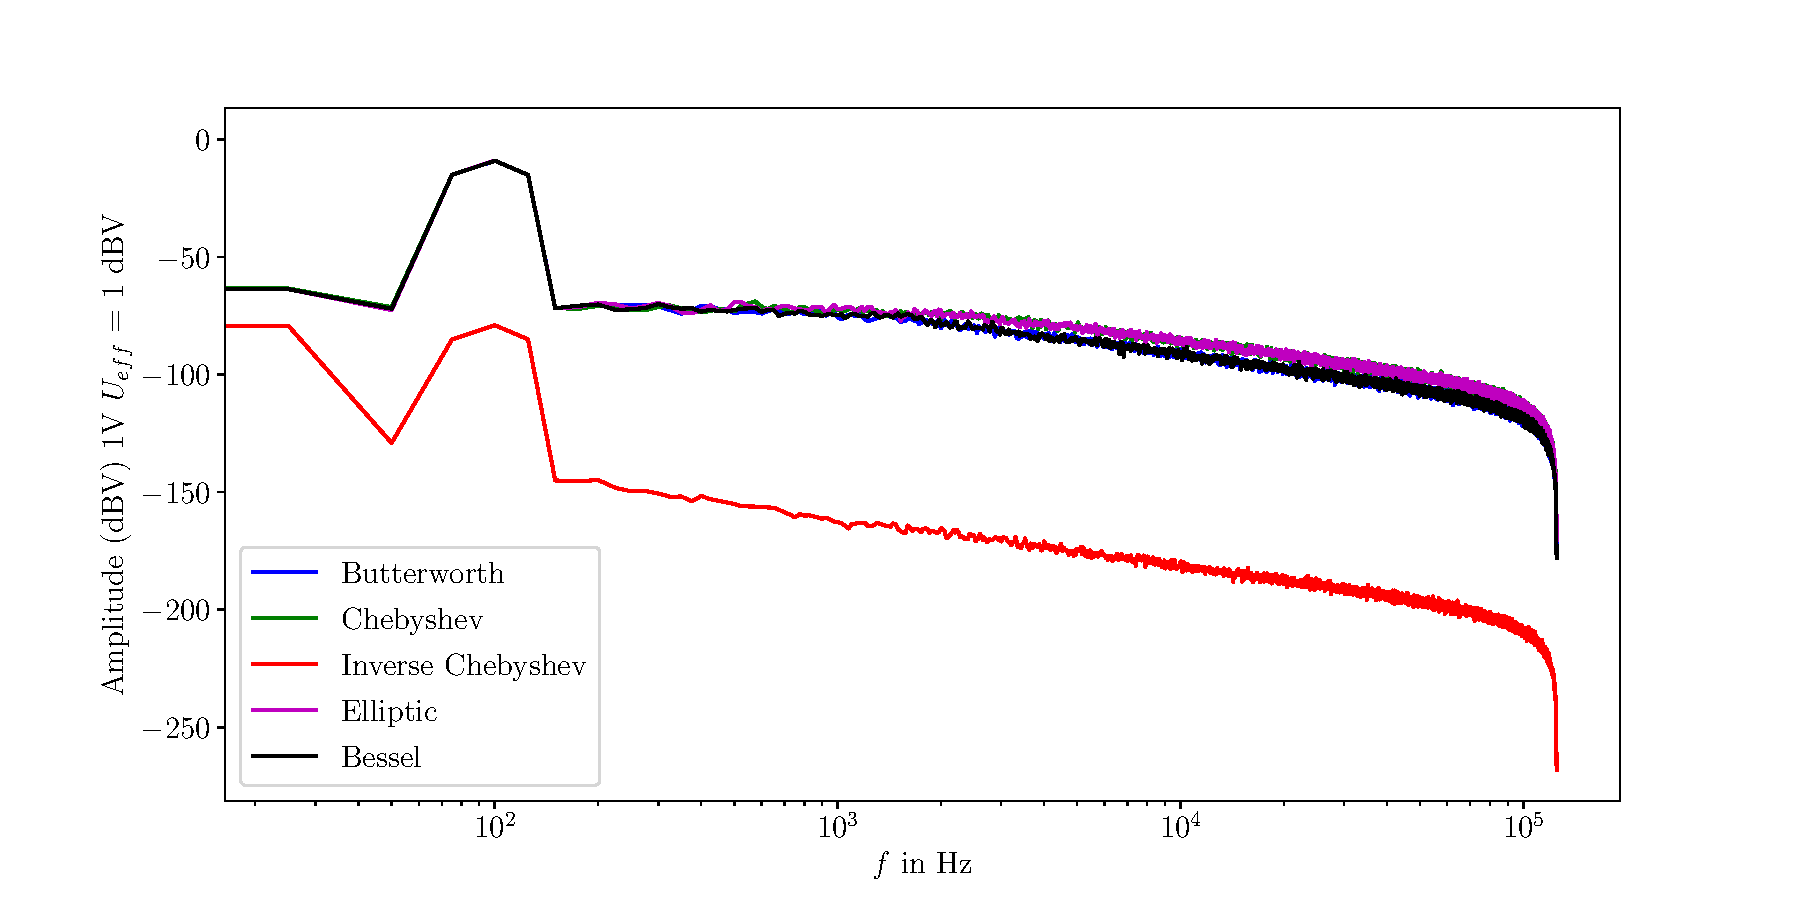
\includegraphics[width=\textwidth]{Paul/43aAll.pdf}
    \caption{Fourierspektrum verschiedene Tiefpassfilter}
\end{figure}

\begin{figure}[h]
    \centering
    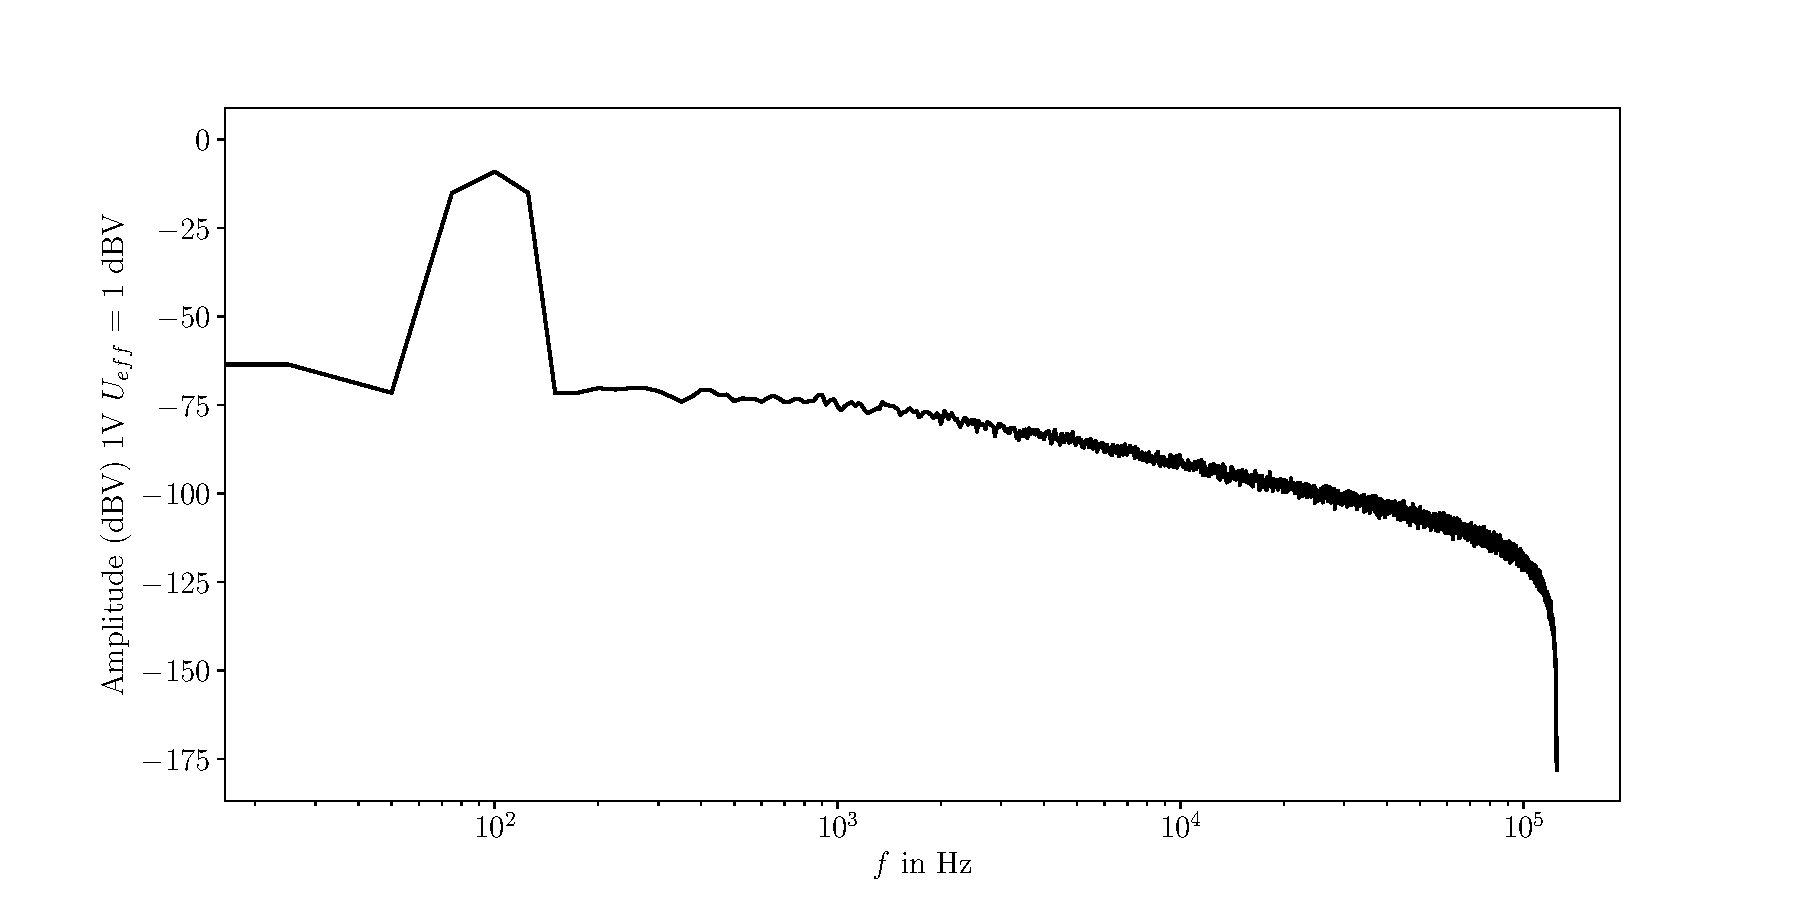
\includegraphics[width=\textwidth]{Paul/43aBu.pdf}
    \caption{Fourierspektrum des Butterworthfilter}
\end{figure}

\begin{figure}[h]
    \centering
    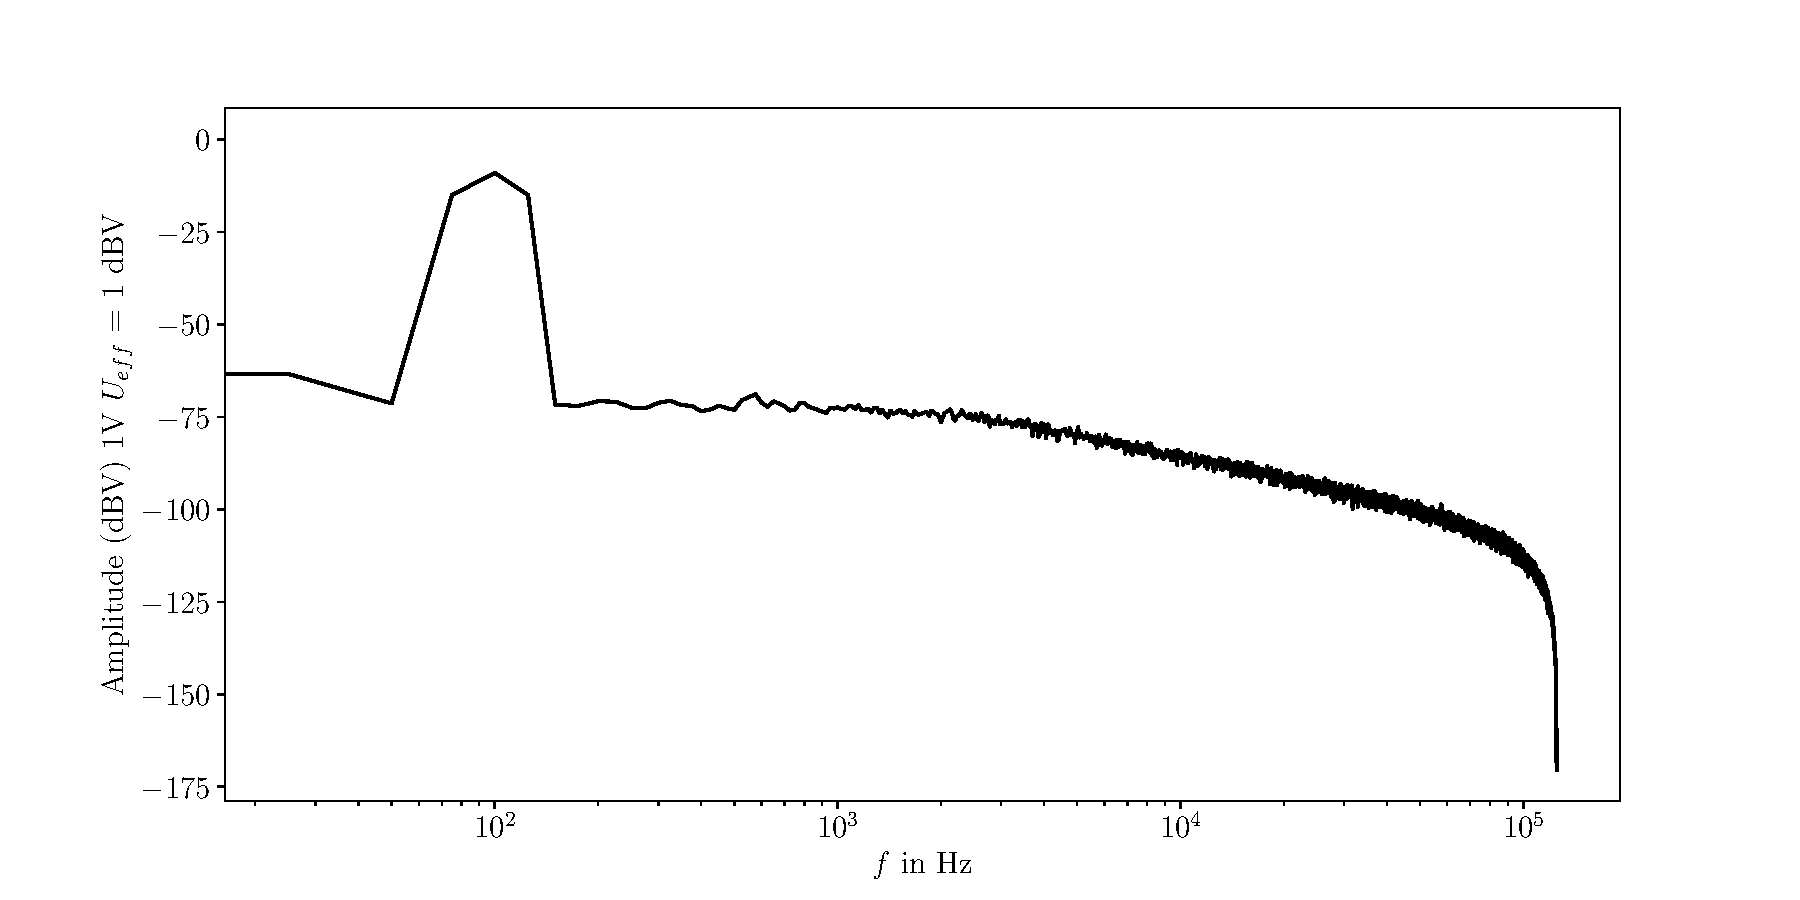
\includegraphics[width=\textwidth]{Paul/43aCh.pdf}
    \caption{Fourierspektrum des Chebyshevfilter}
\end{figure}

\begin{figure}[h]
    \centering
    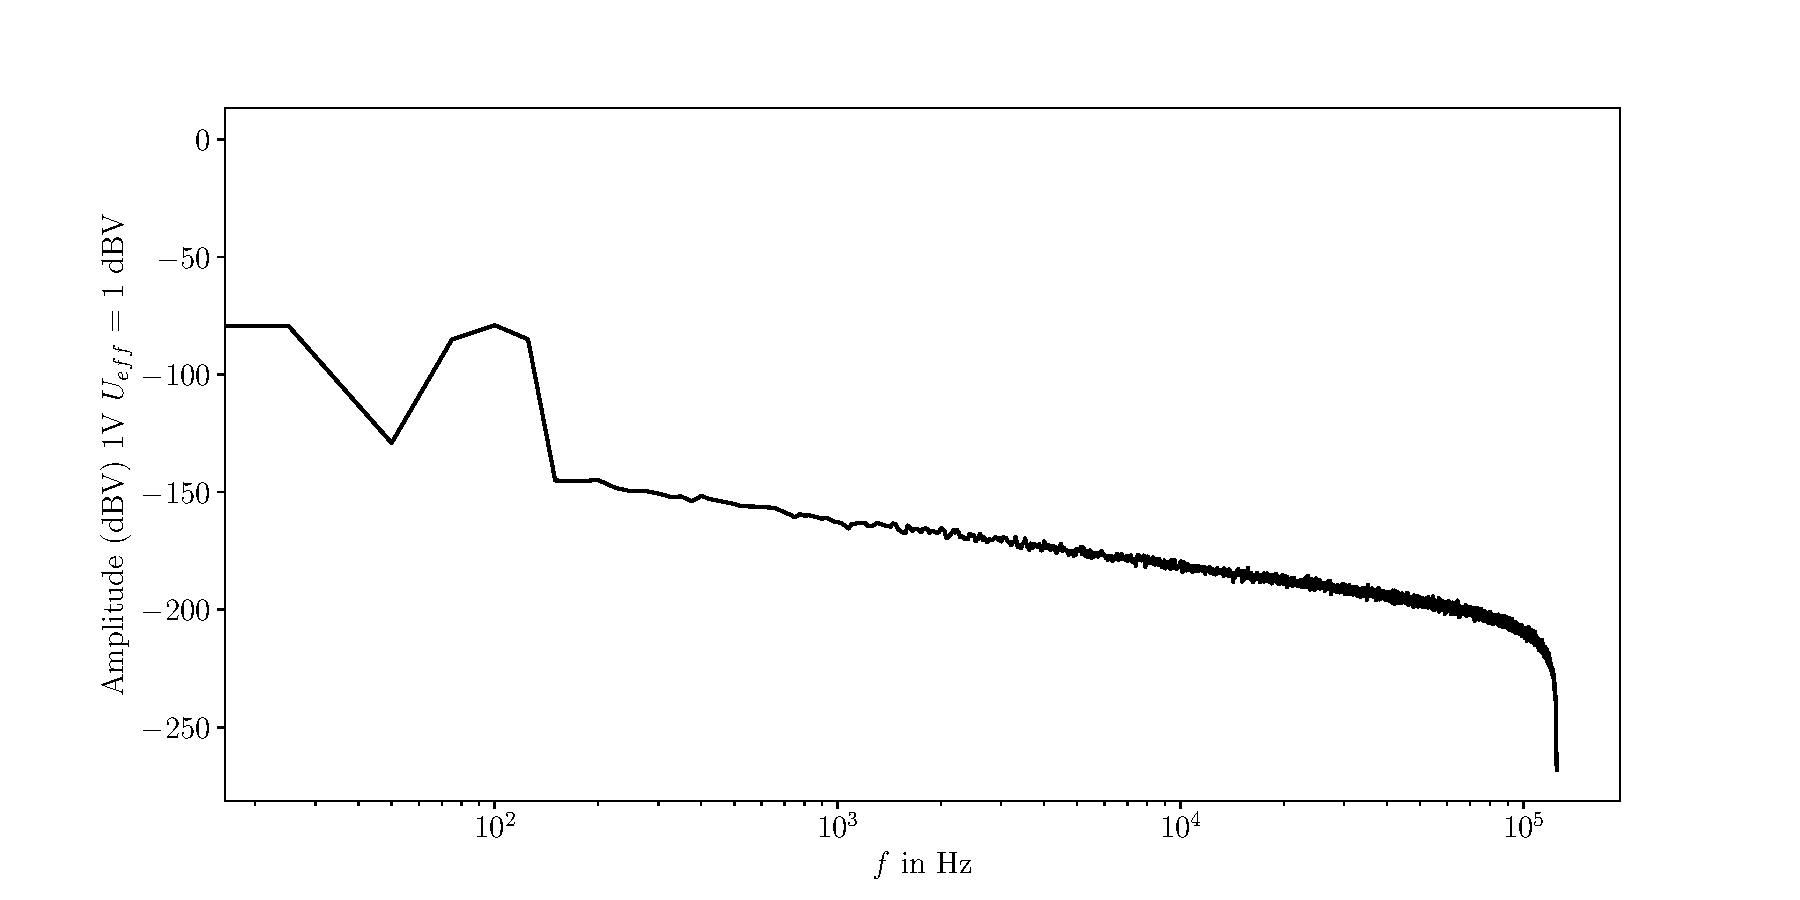
\includegraphics[width=\textwidth]{Paul/43aInCh.pdf}
    \caption{Fourierspektrum des inversen Chebyshevfilter}
\end{figure}

\begin{figure}[h]
    \centering
    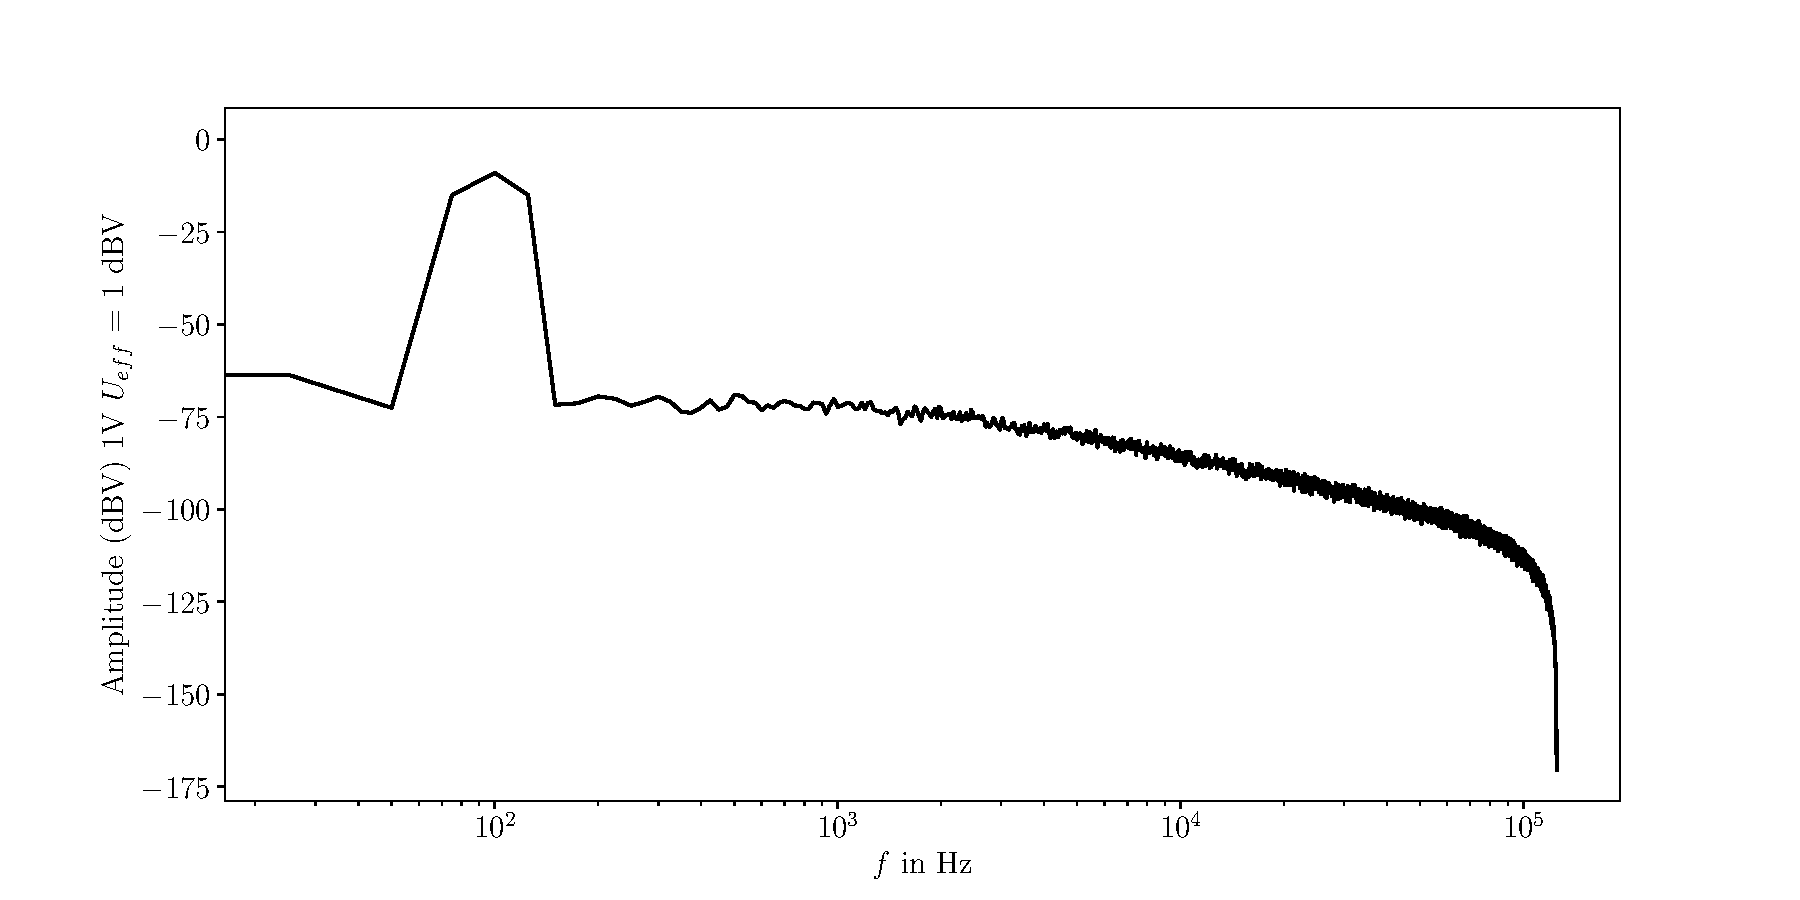
\includegraphics[width=\textwidth]{Paul/43aEl.pdf}
    \caption{Fourierspektrum des Ellipticfilter}
\end{figure}

\begin{figure}[h]
    \centering
    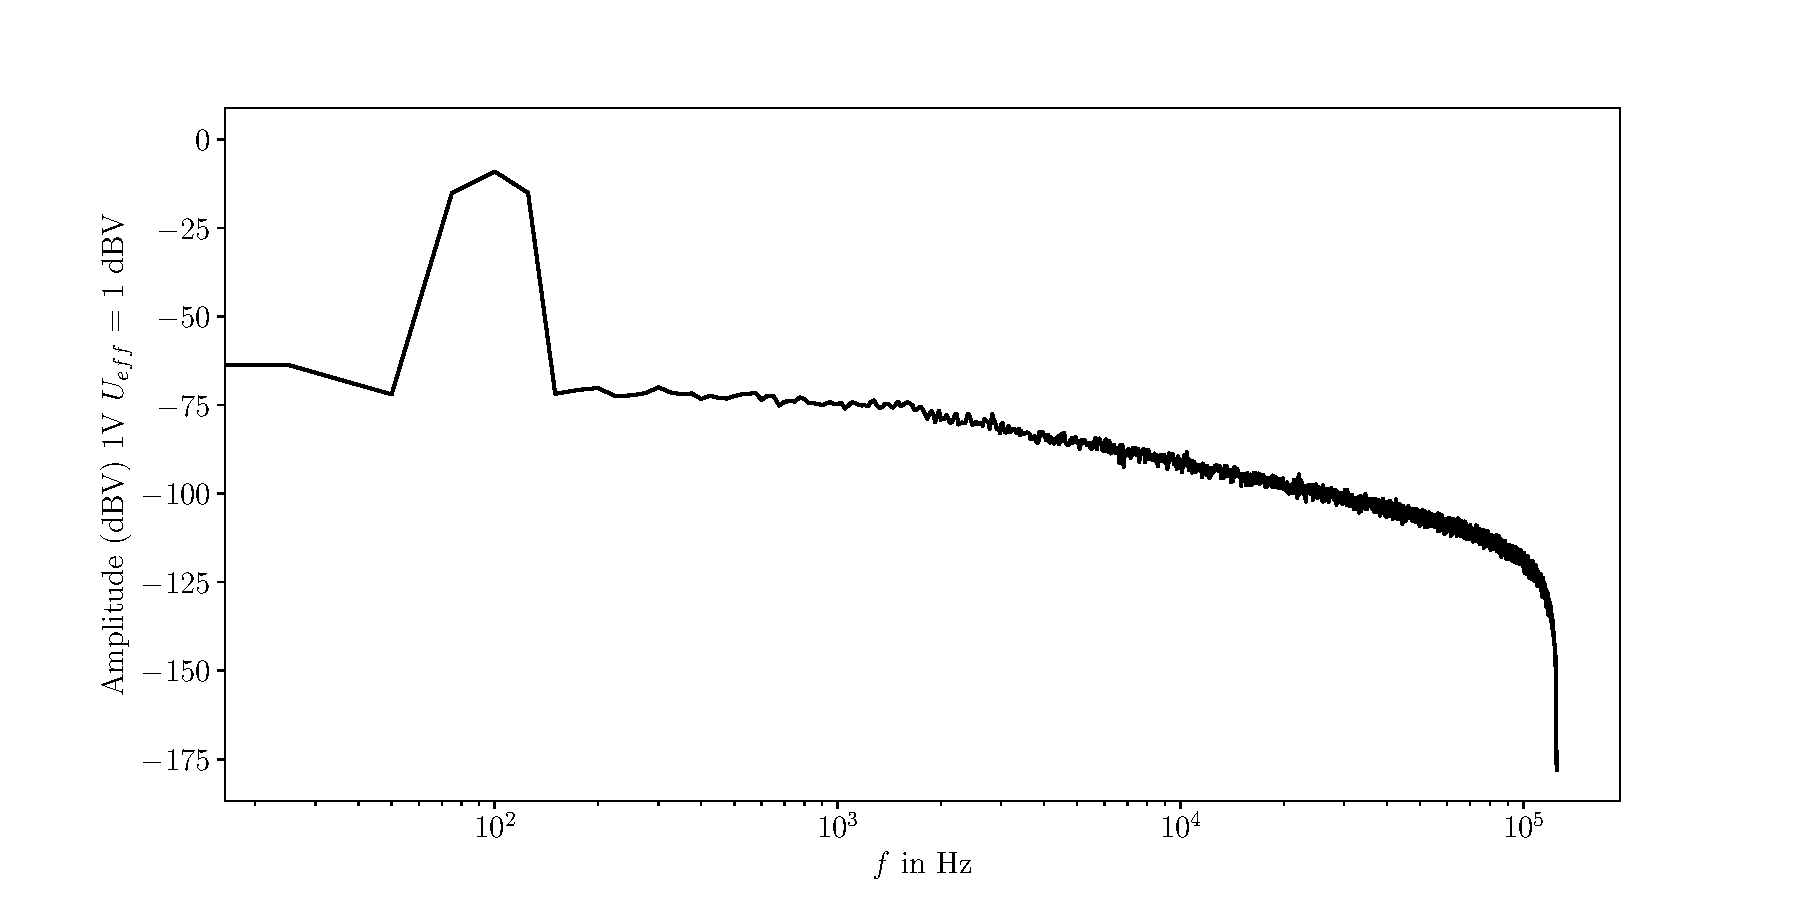
\includegraphics[width=\textwidth]{Paul/43aBe.pdf}
    \caption{Fourierspektrum des Bessselfilter}
\end{figure}


\subsection{Filterwirkung auf Rechtecksignal}



\subsection{Bandpass 4. Ordnung}


\subsection{Einfluss der Ordnung}


\subsection{Analoge vs. digitale Filterung}


\subsection{Vergleich Filterung und Mittelung}